\chapter{Open heavy-flavour production in proton-proton collisions}\label{ch:openHF}

Open heavy-flavour hadrons, composed of a heavy quark (charm or beauty) along with lighter quarks, are exclusively formed in high-momentum transfer processes due to the large masses of approximately 1.3 \gevcc and 4.2 \gevcc~\cite{pdg} for charm and beauty quarks, respectively. As a result, heavy quarks are created in the early stages of the collision, and their production cross-section in the partonic interaction can be evaluated perturbatively using QCD. Studying the production of open heavy-flavour hadrons in proton-proton (pp) collisions not only provides a crucial test of the perturbative QCD framework, but also allows to set constraints on heavy-quark hadronisation models. Furthermore, measurements in proton-proton collisions, where the production of an extended deconfined medium is not expected, are a necessary reference for the study of heavy-ion collisions, where the properties of the QGP can be investigated. 

\section{Factorisation theorem}
The production of open heavy-flavour hadrons in proton-proton collisions can be described using the factorisation theorem~\cite{Collins:1989gx}, which allows for the separation of short-distance, perturbative behaviour from long-distance, non-perturbative phenomena. The total production cross-section can be expressed as
\begin{equation}\label{eq:pp_xsec}
    \sigma_{\text{pp}}^\mathrm{H} = \sum_\mathrm{a,b = g, q, \overline{q}} \int \de x_1 \de x_2 f_\mathrm{a/A}(x_1,\mu_\mathrm{F}^2) f_\mathrm{b/B}(x_2,\mu_\mathrm{F}^2) \hat{\sigma}_\mathrm{ab \rightarrow Q\overline{Q}} (x_1,x_2,\mu_\mathrm{F}^2,\mu_\mathrm{R}^2) D_\mathrm{Q\rightarrow H_Q}(z,\mu_\mathrm{F}^2) \quad ,
\end{equation}
i.e., the convolution of: i) the Parton Distribution Functions (PDFs) $f_\mathrm{a/A}(x_1,\mu_\mathrm{F}^2)$ and $f_\mathrm{b/B}(x_2,\mu_\mathrm{F}^2)$, describing the initial-state probability of finding a parton a in the proton A carrying a fraction $x_1$ of the proton's momentum, and a parton b in the proton B carrying a fraction $x_2$ of its momentum, respectively; ii) the hard partonic scattering cross-section $\hat{\sigma}_\mathrm{ab \rightarrow Q\overline{Q}} (x_1,x_2,\mu_\mathrm{F}^2,\mu_\mathrm{R}^2)$, defining the probability of producing the $\mathrm{Q\overline{Q}}$ final state from the collision of partons a and b, where Q is either a charm or beauty quark; and iii) the Fragmentation Functions (FFs) $D_\mathrm{Q\rightarrow H_Q}(z,\mu_\mathrm{F}^2)$, which describe the probability of the heavy quark Q to fragment into a heavy-flavour hadron $\mathrm{H_Q}$ carrying a fraction of the parent parton momentum $z$. $\mu_\mathrm{F}$ and $\mu_\mathrm{R}$ are the factorisation and renormalisation scales, respectively. The former is the scale at which the non-perturbative processes are separated from the perturbative ones, while the latter is the scale at which the ultraviolet divergences, emerging from the calculations of scattering amplitudes involving loop diagrams, are subtracted. While the PDFs and FFs are non-perturbative quantities, parametrised from experimental data and regarded as universal across different collision systems, the hard partonic scattering cross-section can be perturbatively calculated using QCD, but needs specific evaluations for each process. 

The factorisation theorem has been widely employed to describe the production of open heavy-flavour hadrons in proton-proton collisions, and has proven to be successful in modeling experimental data. Figure~\ref{fig:ppDmeson} shows the production cross-section of prompt and non-prompt $\mathrm{D^0}$-mesons in proton-proton collisions at $\sqrt{s} = 5.02$~\tev measured at midrapidity ($\lvert y\rvert<0.5$) as a function of the transverse momentum (\pt) by the ALICE Collaboration~\cite{ALICE:2021mgk}, compared to Fixed-Order plus Next-to-Leading Logarithms (FONLL) perturbative QCD predictions~\cite{Cacciari:1998it} combined with the \textsc{Pythia}~8~\cite{Sjostrand:2014zea} event generator for the $\mathrm{H_b \rightarrow D^0+X}$ decay kinematics. The calculation is performed at next-to-leading order, including all the $\als^2$ and $\als^3$ terms, with the resummation of the next-to-leading logarithmic terms. These include terms of the form $\alpha_s^2\alpha_s^k\log^k(\pt/m)$ and $\alpha_s^3\alpha_s^k\log^k(\pt/m)$, where $m$ is the heavy-quark mass. The term \emph{prompt} refers to charm-hadrons directly produced in the hadronisation of a charm quark or through the strong decay of a directly produced excited charm-hadron or charmonium state, while \emph{non-prompt} charm hadrons are produced in the decay of a hadron containing a beauty quark. The FONLL predictions are in good agreement with the non-prompt $\mathrm{D^0}$-meson production cross-section, whereas the prompt contribution lies at the upper edge of the theoretical uncertainty band, albeit being described within the uncertainties. Similar trends are observed in the production of other open heavy-flavour hadrons across different experimental facilities, such as the Tevatron~\cite{CDF:2003vmf}, RHIC~\cite{STAR:2012nbd}, and LHC~\cite{ALICE:2021mgk}.

\begin{figure}[htb]
    \centering
    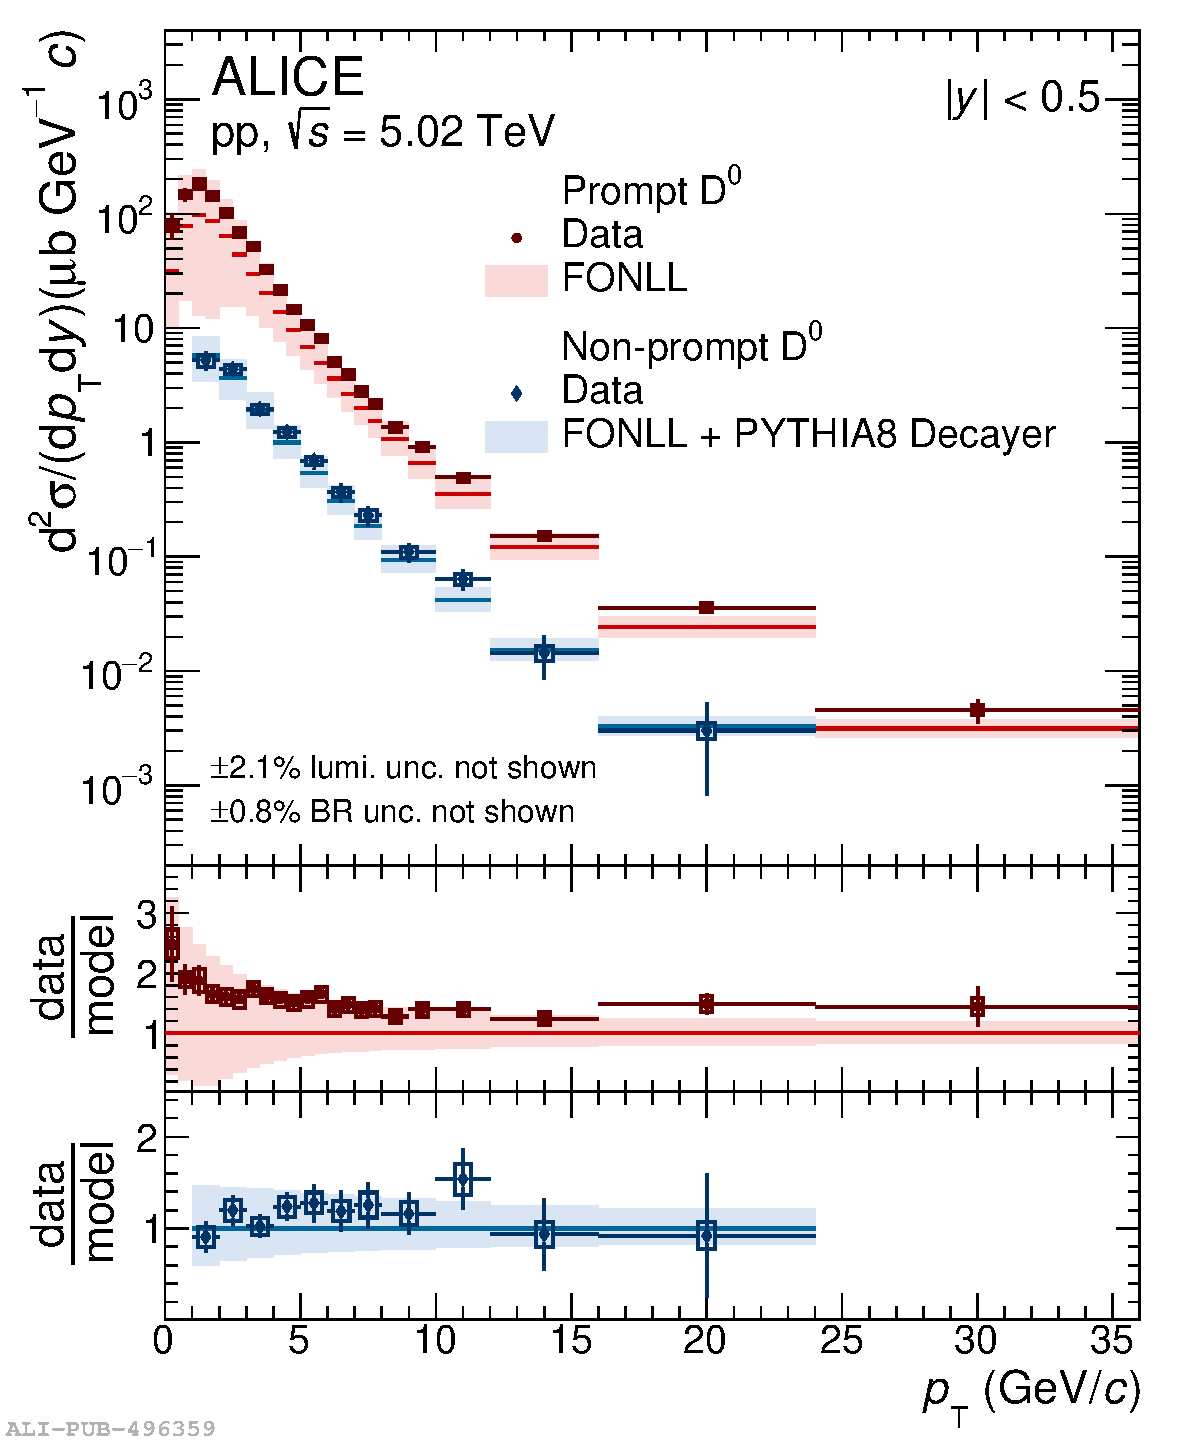
\includegraphics[width=0.6\linewidth]{Figures/Chapter 2/CrossSectionD0_Prompt_NonPrompt_pp5TeV_vsFONLL_Pythia8_BRnative_1.pdf}
    \caption{\pt-differential production cross-section of prompt and non-prompt $\mathrm{D^0}$-mesons measured at midrapidity ($\lvert y\rvert<0.5$) in pp collisions by the ALICE Collaboration at $\sqs=5.02$~\tev~\cite{ALICE:2021mgk} compared to predictions obtained with FONLL calculations~\cite{Cacciari:1998it} combined with \textsc{Pythia}~8~\cite{Sjostrand:2014zea} for the $\mathrm{H_b \rightarrow D^0+X}$ decay kinematics. Figure taken from Ref.~\cite{ALICE:2021mgk}}
    \label{fig:ppDmeson}
\end{figure}

\subsection{Parton Distribution Functions}
\subsubsection{Deep inelastic scattering}
The PDFs are non-perturbative quantities describing the probability of finding a parton carrying a fraction $x$ of the proton's momentum in the initial state of a process. The first experimental evidence revealing the partonic structure of the proton emerged from deep inelastic scattering experiments carried out at the Stanford Linear Accelerator Center (SLAC) in the 1960s~\cite{Friedman:1972sy}, where an electron was scattered off a proton with momentum $P$
, and the transferred momentum $q$ was measured. The cross-section for deep inelastic scattering can be defined in terms of the Lorentz invariant variables $Q^2 = -q^2$ and $x = \frac{Q^2}{2P\cdot q}$, yielding
\begin{equation*}
    \frac{\de^2\sigma}{\de x \de Q^2} = \frac{4\pi\alpha^2}{xQ^4} \left[ \left(1-y\right)F_2(x,Q^2) - xy^2F_1(x,Q^2) \right]\quad ,
\end{equation*}
where $y=Q^2/(sx)$, $s = (P+p_\mathrm{e})^2$ denotes the centre-of-mass energy of the electron-proton system, and the structure functions $F_1(x,Q^2)$ and $F_2(x,Q^2)$ represent an extension of the form factors for elastic scattering.
The first measurements of high-energy inclusive inelastic scattering experiments were performed using a 20~GeV linear accelerator at SLAC, and showed that the structure functions $F_1(x,Q^2)$ and $F_2(x,Q^2)$ were independent of $Q^2$ at fixed $x$ within the studied $1<~Q^2~<~10$~\gevcc range. This was in contrast with the behavior observed for the proton elastic form factors, where a decrease of two orders of magnitude was observed within the same $Q^2$ interval. This independence of the structure functions from $Q^2$ in deep inelastic scatterings was predicted by Bjorken in 1968 for $Q^2 \rightarrow \infty$~\cite{Bjorken:1968dy}, and is known as \emph{Bjorken scaling}. A physical interpretation of this phenomenon arrived just one year later, in 1969, with Feynman's parton model~\cite{Feynman:1969ej}, which described the interaction in terms of elastic scattering of the probe off a point-like constituent (parton) within the proton. This model explains the scale-invariance property of the proton structure functions, as the scattering centres are assumed to be structure-less. In this picture, the Bjorken variable $x$ acquires a new interpretation as the fraction of the proton momentum carried by the struck parton. The parton model also offers a straightforward definition of the structure functions in terms of the parton distribution functions $f_\mathrm{a}(x)$:
\begin{equation*}
    F_2(x,Q^2) = \sum_\mathrm{a} e_\mathrm{a}^2 x f_\mathrm{a}(x)\quad ,
\end{equation*}
where the sum is over partons with electric charge $e_\mathrm{a}$, and $f_\mathrm{a}$ are unknown, but universal functions for a given hadron, describing the probability of finding a parton of type a with a fraction $x$ of the proton's momentum. 

To explore the spin properties of the partons, the structure functions $F_1$ and $F_2$ were studied at different centre-of-mass energies. By investigating the relationship between the two structure functions, it was established that the partons have spin 1/2, as the Callan-Gross relation~\cite{Callan:1969uq}, which holds true for point-like Dirac particles, was found to be satisfied:
\begin{equation*}
    F_2(x,Q^2) = 2x F_1(x,Q^2)\quad .
\end{equation*}

In the next years, it became clear that additional constituents within the proton carry momentum but lack electric or weak charge, as the so-called momentum sum rule was not saturated by the measured PDFs in electron and neutrino scatterings. This missing momentum was attributed to gluons, which were discovered in the 1970s and are the field quanta of the strong force.

\subsubsection{Bjorken scaling violation}
\begin{figure}[htb]
    \centering
    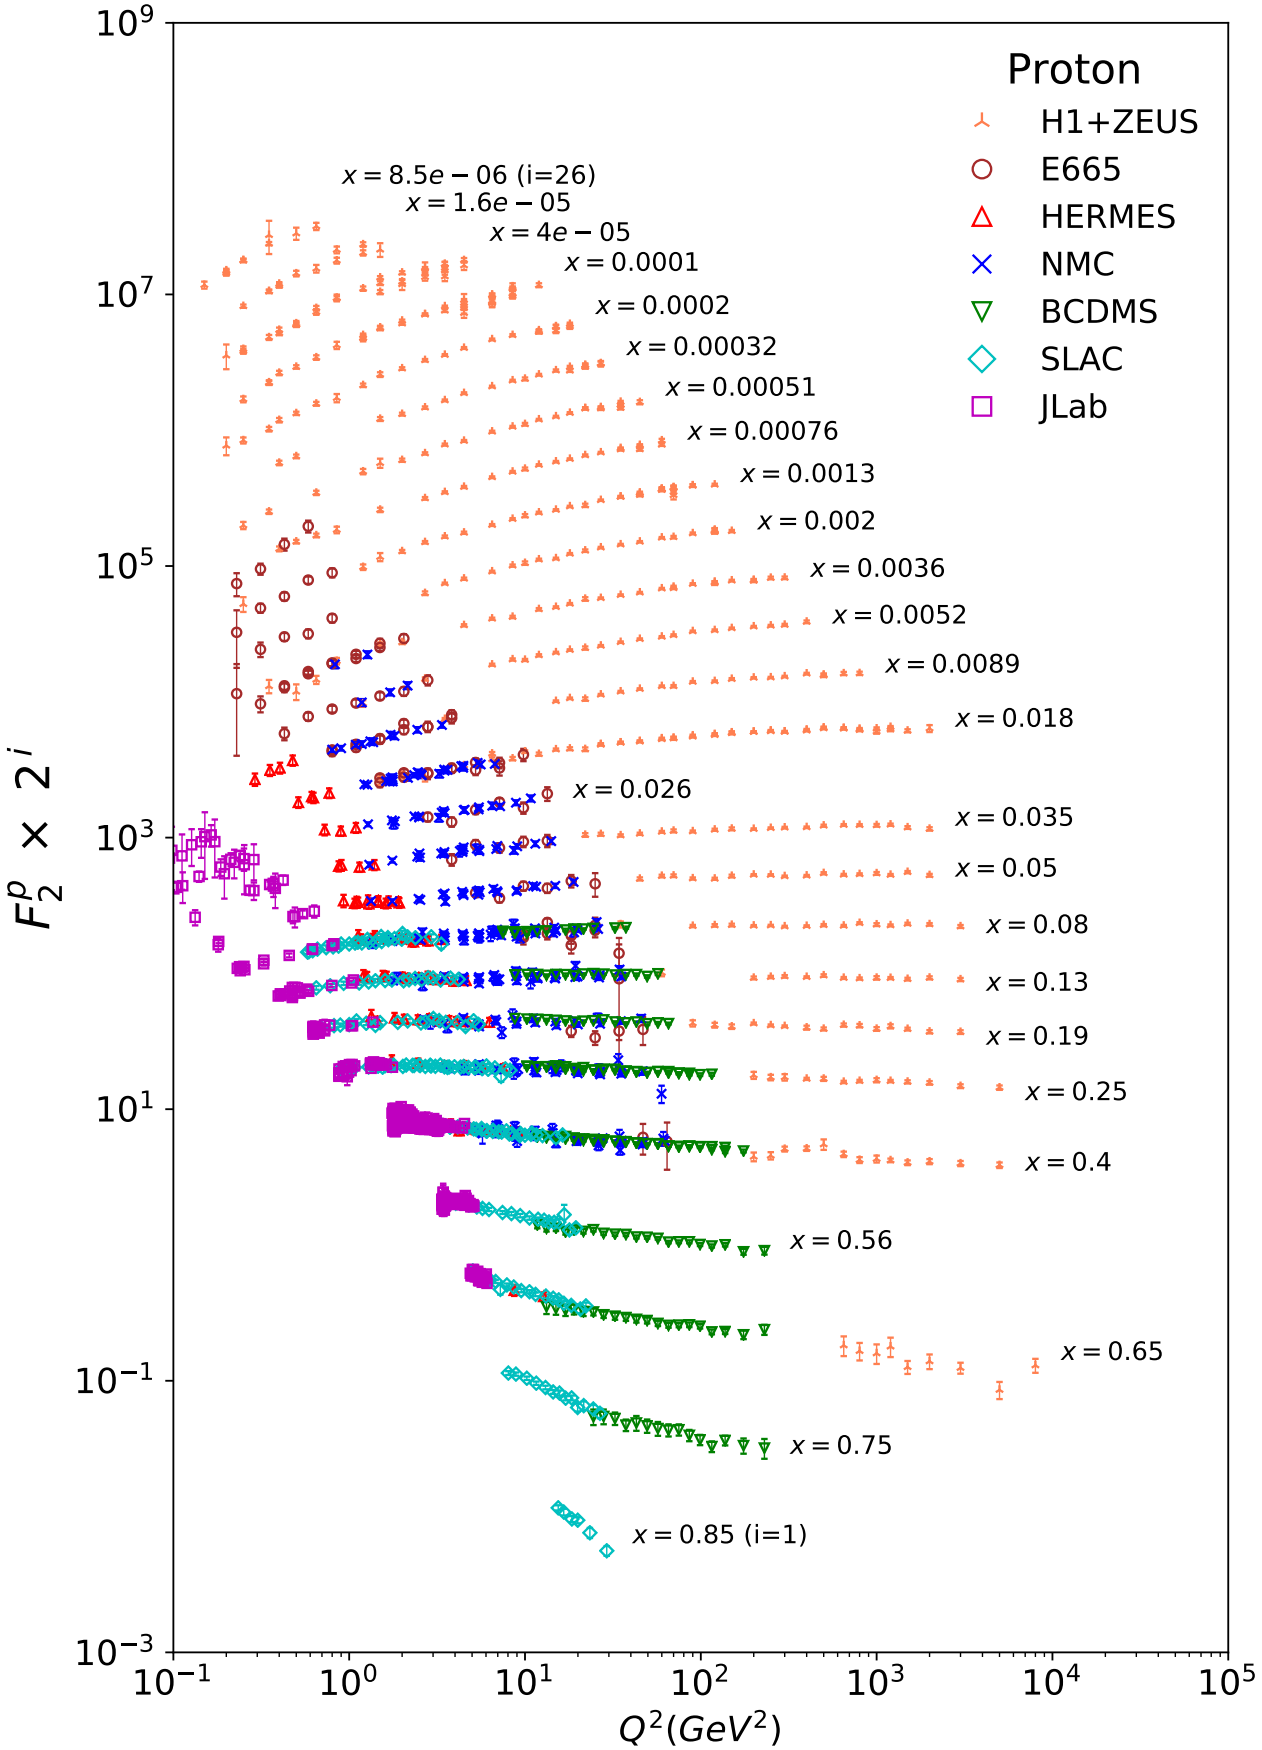
\includegraphics[width=0.6\linewidth]{Figures/Chapter 2/F2Results.png}
    \caption{The proton structure function $F^p_2$ measured in electromagnetic scattering of electrons and positrons on protons, and for electrons/positrons and muons on a fixed target~\cite{pdg}.}
    \label{fig:scaling_violation}
\end{figure}
By the late 1970s, measurements of the structure functions at larger $Q^2$ values taken at CERN and DESY revealed that Bjorken scaling was violated, i.e., the structure functions were not $Q^2$ independent. Figure~\ref{fig:scaling_violation} shows measurements of the proton structure functions $F_2(x,Q^2)$ as a function of $Q^2$ for various values of $x$ taken from different experiments~\cite{pdg}. It is clear from the plot that structure functions present an increasing trend as a function of $Q^2$ at low $x$, and a decreasing trend as a function of $Q^2$ at high $x$. 

The parton model fails to explain this behaviour, as it relies on the assumption that the transferred energy is sufficiently large to neglect the proton and its constituents' masses, as well as the interactions among partons. In particular, the partons' transverse momentum with respect to the proton momentum is neglected. The key to understanding Bjorken scaling violation comes from QCD and the realisation that the parton's transverse momentum is not necessarily restricted to be small. A quark, for instance, can emit a gluon and acquire large transverse momentum $k_T$ with a probability proportional to $\als \de k_T/k_T^2$ at large $k_T$. The integral extends up to the kinematic limit $k_T\sim Q^2$, giving rise to contributions proportional to $\als\mathrm{log}Q^2$, which break the scaling. The evolution of PDFs with $Q^2$ from a parametrisation at a given $Q^2_0$ can be perturbatively described using the Dokshitzer-Gribov-Lipatov-Altarelli-Parisi (DGLAP) evolution equations~\cite{Gribov:1972ri,Dokshitzer:1977sg,Altarelli:1977zs}, which require the introduction of a new arbitrary scale, at which the factorisation of the non-perturbative processes happens: the factorisation scale $\mu_\mathrm{F}$. There exists a wide range of PDF parametrisations, such as the NNPDF~\cite{NNPDF:2021njg}, CTEQ~\cite{Dulat:2015mca}, and MMHT~\cite{Harland-Lang:2014zoa}, which are determined from global fits to a wide range of experimental data, including deep inelastic scattering, Drell-Yan, and jet production.
\subsection{Partonic cross-section}\label{sec:partonic_cross_section}
\begin{figure}[htb]
    \centering
    \begin{tikzpicture}
      \begin{feynman}
        \vertex (a);
        \vertex [above=1cm of a] (b) {q};
        \vertex[below=1cm of a] (c) {$\overline{\mathrm{q}}$};
        \vertex[right=1cm of a] (d);
        \vertex[right=0.7cm of d] (e);
        \vertex[right=1.3cm of e] (f);
        \vertex[right=0.7cm of f] (g);
        \vertex[right=1cm of g] (h);
        \vertex[above=1cm of h] (i) {Q};
        \vertex[below=1cm of h] (j) {$\overline{\mathrm{Q}}$};
        \diagram* {
            (b) -- [fermion] (d) -- [fermion] (c),
            (d) -- [gluon] (e),
            (e) -- [gluon,  in=90, out=90, looseness=1.7] (f) -- [gluon,  in=-90, out=-90, looseness=1.7] (e),
            (f) -- [gluon] (g),
            (j) -- [fermion] (g) -- [fermion] (i),
        };
      \end{feynman}
    \end{tikzpicture}\quad
    \begin{tikzpicture}
        \begin{feynman}
          \vertex (a);
          \vertex [above=1cm of a] (b) {q};
          \vertex[below=1cm of a] (c) {$\overline{\mathrm{q}}$};
          \vertex[right=1cm of a] (d);
          \vertex[right=0.7cm of d] (e);
          \vertex[right=1.3cm of e] (f);
          \vertex[right=0.7cm of f] (g);
          \vertex[right=1cm of g] (h);
          \vertex[above=1cm of h] (i) {Q};
          \vertex[below=1cm of h] (j) {$\overline{\mathrm{Q}}$};
          \diagram* {
              (b) -- [fermion] (d) -- [fermion] (c),
              (d) -- [gluon] (e),
              (e) -- [fermion,  in=90, out=90, looseness=1.7] (f) -- [fermion,  in=-90, out=-90, looseness=1.7] (e),
              (f) -- [gluon] (g),
              (j) -- [fermion] (g) -- [fermion] (i),
          };
        \end{feynman}
      \end{tikzpicture}

    \vspace*{0.5cm}
    \begin{tikzpicture}
        \begin{feynman}
          \vertex (a);
          \vertex [above=1cm of a] (b) {q};
          \vertex[below=1cm of a] (c) {$\overline{\mathrm{q}}$};
          \vertex[right=1cm of a] (d);
          \vertex[right=1cm of d] (e);
          \vertex[right=1cm of e] (f);
          \vertex[above=1cm of f] (g) {Q};
          \vertex[below=1cm of f] (h) {$\overline{\mathrm{Q}}$};
          \vertex[right=0.5cm of e] (i);
          \vertex[below=0.5cm of i] (j);
          \diagram* {
              (b) -- [fermion] (d) -- [fermion] (c),
              (d) -- [gluon] (e),
              (h) -- [fermion] (e) -- [fermion] (g),
              (j) -- [gluon, edge label = g] (f),

          };
        \end{feynman}
      \end{tikzpicture}\quad
      \begin{tikzpicture}
        \begin{feynman}
            \vertex (a);
            \vertex [above=1cm of a] (b) {q};
            \vertex[below=1cm of a] (c) {$\overline{\mathrm{q}}$};
            \vertex[right=1cm of a] (d);
            \vertex[right=1cm of d] (e);
            \vertex[right=1cm of e] (f) ;
            \vertex[above=1cm of f] (g) {Q};
            \vertex[below=1cm of f] (h) {$\overline{\mathrm{Q}}$};
            \vertex[right=0.5cm of e] (i);
            \vertex[below=0.5cm of i] (j);
          \diagram* {
              (b) -- [gluon] (d) -- [gluon] (c),
              (d) -- [gluon] (e),
              (h) -- [fermion] (e) -- [fermion] (g),
              (j) -- [gluon, edge label = g] (f),

          };
        \end{feynman}
      \end{tikzpicture}\quad
      \begin{tikzpicture}
        \begin{feynman}
          \vertex (a) {g};
          \vertex[above=0.25cm of a] (spacing) {$ $  }; 
          \vertex[right=1.25cm of a] (b);
          \vertex[right=1.45cm of b] (c) {q};
          \vertex[below=1.75cm of a] (d) {q};
          \vertex[right=1.25cm of d] (e);
          \vertex[right=0.75cm of e] (f);
          \vertex[right=1cm of f] (g);
          \vertex[above=0.3cm of g] (h) {Q};
          \vertex[below=0.3cm of g] (j) {$\overline{\mathrm{Q}}$};
          \diagram* {
                (a) -- [gluon] (b),
                (d) -- [fermion] (e) -- [fermion] (b) -- [fermion] (c),
                (e) -- [gluon] (f),
                (j) -- [fermion] (f) -- [fermion] (h),
          };
        \end{feynman}
      \end{tikzpicture}\quad
    \caption{Feynman diagrams contributing to the first order corrections of the heavy-flavour production cross-section calculations.}
    \label{fig:NLO_diagrams}
\end{figure}

\begin{sloppypar}
Because of their large masses, heavy quarks can only be produced through hard-scattering processes, characterised by momentum transfers of the order of \mbox{$Q^2 \geq 4m^2_\mathrm{b,c}$}. In this regime, the strong coupling constant is significantly smaller than unity, allowing for the perturbative calculation of the heavy quark production cross-section from partonic scattering using QCD. While predictions at next-to-next-to-next-to-leading order (N$^3$LO) are available for certain processes, such as Higgs production~\cite{Anastasiou:2015vya, Anastasiou:2016cez}, the current state-of-the-art calculations for charm-quark production are at next-to-leading order (NLO) with all-order resummation to next-to-leading logarithmic (NLL) accuracy in the limit where the \pt of a heavy quark is much larger than its mass~\cite{Cacciari:1998it}. The contributions arising at the NLO include 1-loop virtual corrections to the Born process and real emission of a gluon or a quark-antiquark pair, and are depicted in Fig~\ref{fig:NLO_diagrams}. Next-to-next-to-leading order (NNLO) QCD radiative corrections to the production of bottom-quark pairs have also been computed~\cite{Catani:2020kkl}.
\end{sloppypar}

\subsection{Fragmentation Functions}
\begin{sloppypar}
Quarks and gluons produced in hard-scattering processes ultimately give rise to colourless observable hadrons. The associated process, known as hadronisation, is non-perturbative since the partonic processes involved are characterised by relatively small energy scales ($\sim\Lambda_\mathrm{QCD}$), where the strong coupling constant is large. The hadronisation process is described by the Fragmentation Functions (FFs) $D_\mathrm{Q\rightarrow H_Q}(z,\mu_\mathrm{F}^2)$, which parametrise the probability of the heavy quark Q to fragment into a heavy-flavour hadron $\mathrm{H_Q}$ with a fraction of the parent parton momentum $z$. They provide a simple ``effective" description of the parton-to-hadron transition by mapping the quark-momentum-differential cross-section into the hadron-momentum differential one. FFs are typically determined from experimental data, usually by analyzing the final-state hadrons produced in electron-positron collisions where the initial momenta are well-known. These FFs are then applied in the evaluation of cross-sections in other colliding systems, assuming that the relevant hadronisation processes are “universal”, i.e., independent of the collision energy and system. This assumption implies the hypothesis of \emph{independent fragmentation}, which states that the hadronisation of the parton produced in the hard-scattering process is independent of the production mechanism and the partonic environment which surrounds it. Differently from the fragmentation of light quarks and gluons, kinematic considerations on heavy-quark fragmentation~\cite{Bjorken:1977md,Suzuki:1977km} suggest that heavy hadrons tend to carry a larger fraction of the parent parton momentum. Fragmentation functions for heavy quarks are therefore shifted towards higher values of $z$ compared to those of light quarks and gluons~\cite{Peterson:1982ak}. Many FFs have been determined from global fits to data, such as the NNFF1.1h~\cite{Bertone:2018ecm}, DSS~\cite{deFlorian:2007aj}, and KKP~\cite{Kniehl:2000fe} parametrisations for light flavours, and typically differ in the data sets used for the fit, the treatment of the data, and the functional form of the FFs. Parametrisations for heavy quark fragmentation include that of Peterson et al.~\cite{Peterson:1982ak}, Kartvelishvili et al.~\cite{Kartvelishvili:1977pi}, and Breetan et al.~\cite{Braaten:1994bz}. Similarly to PDFs, FFs also evolve with the energy scale of the interaction, and this evolution is described perturbatively by the DGLAP equations. 
\end{sloppypar}

\section{Hadronisation: microscopic and macroscopic descriptions}\label{sec:hadronisation}
Despite being a very powerful effective tool for describing heavy-flavour hadron production, the parametrisation of fragmentation functions used in a factorisation-theorem approach is not the only method used to describe the hadronisation of energetic quarks in high-energy collisions. Over the years, other models have been developed to describe hadron production starting from a partonic stage (e.g., quarks and gluons from the initial hard-scattering process, and those being radiated from the initial partons) and implementing a colour neutralisation procedure that groups quarks and gluons into hadrons.

The standard approach for describing the complex event topologies in these models, which are typically implemented in Monte Carlo event generators, begins with a matrix-element calculation for the production of a few well-separated partons, followed by the application of a parton shower. The \emph{parton shower} provides an approximate perturbative treatment of QCD dynamics, which is then combined with a non-perturbative model for the hadronisation process at a certain infrared cut-off scale, typically taken to be of the order of 1~\gev. The basic idea of the parton shower relies on the Sudakov form factor~\cite{Sudakov:1954sw}, which expresses the probability of a parton not radiating another parton in a given phase space region. If a parton does radiate, the newly-produced parton becomes the source of a new cascade, continuing until the parton shower terminates at the hadronisation scale. At this point, partons are allowed to fragment into hadrons through hadronisation models. 

Although several hadronisation models have been developed, each implementing a different approach to the description of this non-perturbative process, a common feature is the hypothesis of local parton-hadron duality~\cite{Azimov:1984np}, which states that the flow of momentum and quantum numbers at the hadron level tends to follow the flow established at the parton level.

\subsection{Independent fragmentation}\label{sec:independent_fragmentation}
The description of the hadronisation process using FFs relies on the assumption of \emph{independent fragmentation}, i.e., the probability of a parton fragmenting into a hadron is considered independent of the other partons produced in the same collision, effectively considering the hadronisation process as universal, i.e., independent of the collision energy and system. In the original scheme proposed by R. Field and R. Feynman~\cite{Field:1976ve}, the fragmenting quark combines with an antiquark from a $\mathrm{q\overline{q}}$ pair produced from the vacuum to create a meson with energy fraction $z$. The remaining quark, with energy fraction $(1-z)$, fragments in the same way, continuing until an energy cut-off is reached. The probability distribution of $z$ is the fragmentation function. The assumption of independent fragmentation is valid in the case of low-multiplicity \ee collision events, where the number of produced partons is small and no hadronic remnants are present.

However, recent results on the production of strange and heavy-flavour baryons in proton-proton and proton-lead collisions at the LHC~\cite{ALICE:2020wla,ALICE:2024ozd} show that a description of the hadronisation process based on independent fragmentation is not sufficient to describe the data, as it significantly underestimates the baryon production. Figure~\ref{fig:Lambda_c_D0_ee} shows the $\mathrm{\lc/D^0}$ production-yield ratio measured at midrapidity ($\lvert y\rvert<0.5$) in pp collisions at $\sqrt{s} = 5.02$~\tev by the ALICE Collaboration~\cite{ALICE:2020wla} as a function of \pt, compared to theoretical predictions. The predictions are obtained from: i) \textsc{Pythia}~8 with Monash tune~\cite{Skands:2014pea}; ii) HERWIG~7~\cite{Bellm:2015jjp}; iii) POWHEG~\cite{Frixione:2007nw} NLO pQCD calculations, matched with \textsc{Pythia}~6 to generate the parton shower; iv) General-Mass Variable-Flavour-Number Scheme~\cite{Kniehl:2005mk} (GM-VFNS) NLO pQCD calculation with next-to-leading-log resummation. All these models, whose details are described in the following sections, implement fragmentation processes tuned on results of charm production measurements is \ee collisions, and predict an almost \pt-independent $\mathrm{\lc/D^0}$ ratio of around 0.1, significantly underestimating the values measured in pp collisions by a factor of about 5 at low \pt.

\begin{figure}[htb]
  \centering
  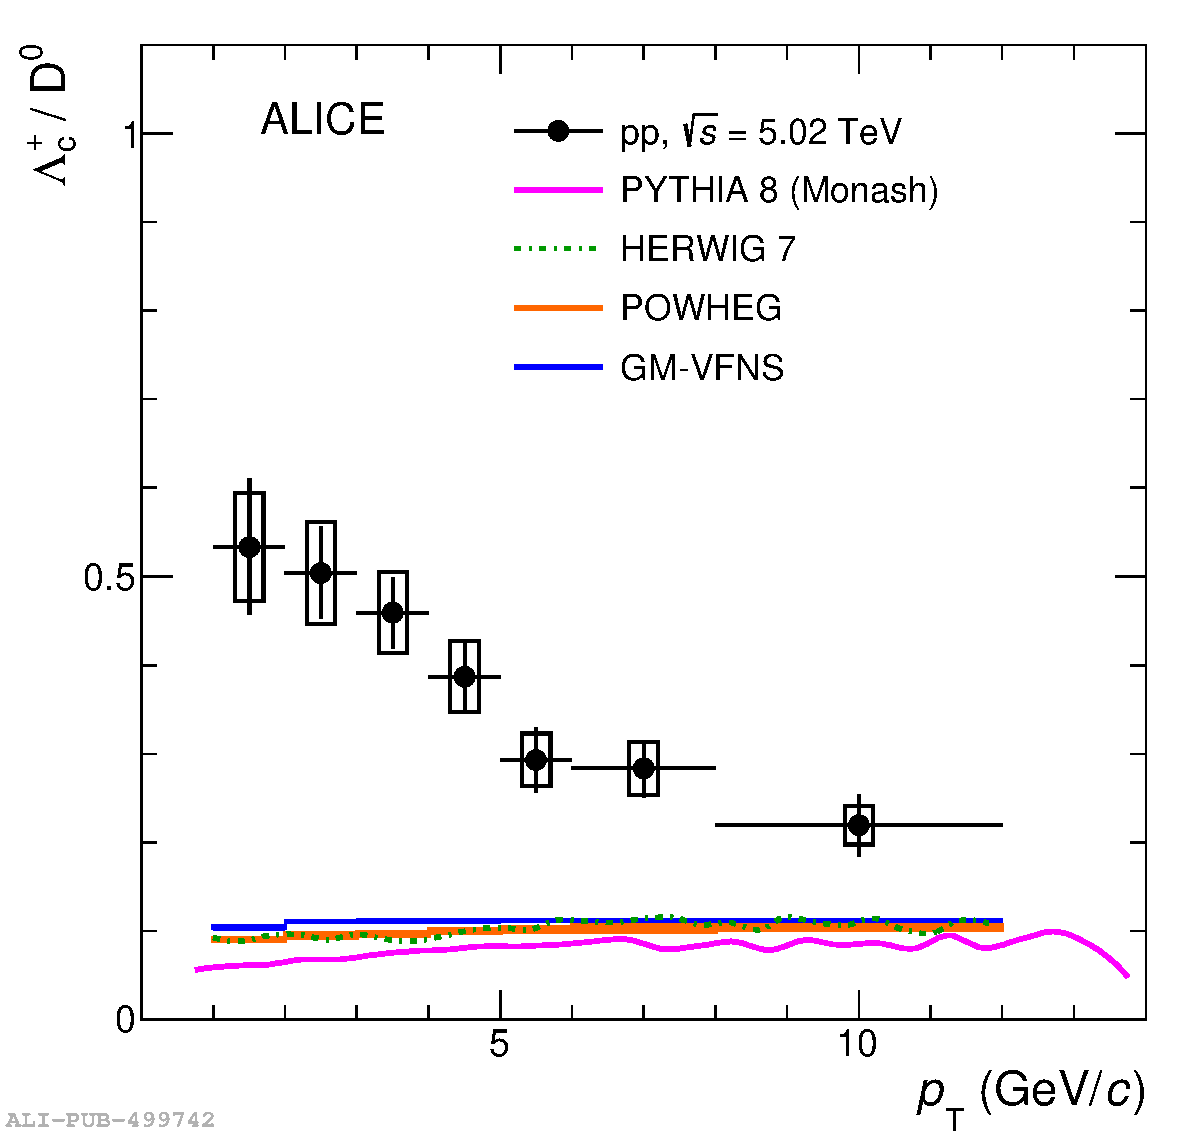
\includegraphics[width=0.7\linewidth]{Figures/Chapter 2/LcD_models_withFFModels_ropes_2.pdf}
  \caption{$\mathrm{\lc/D^0}$ production-yield ratio measured at $\sqrt{s} = 5.02$~\tev by the ALICE Collaboration as a function of \pt, compared to theoretical predictions. Figure taken from Ref.~\cite{ALICE:2020wla}.}
  \label{fig:Lambda_c_D0_ee}
\end{figure}


\subsection{String model}
\begin{figure}[htb]
    \centering
    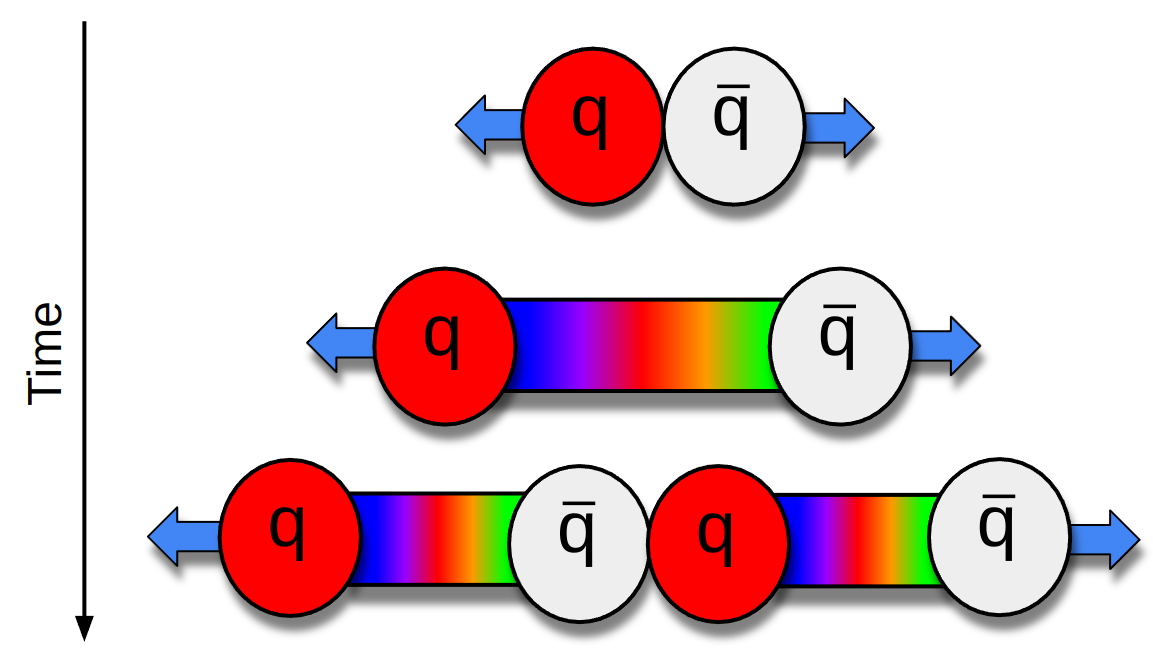
\includegraphics[width=0.7\linewidth]{Figures/Chapter 2/Lund.png}
    \caption{Schematic representation of the Lund string model hadronisation process.}
    \label{fig:Lund}
\end{figure}
The most widely used model for the description of the hadronisation process in Monte Carlo event generators is the Lund string model~\cite{Andersson:1983ia}, employed in the \textsc{Pythia} event generator~\cite{Bierlich:2022pfr}. In this model, the strong force between quarks and gluons is modelled in terms of a colour string with energy given by the Cornell potential~\cite{Eichten:1974af},
\begin{equation*}
    V(r) = -\frac{A(r)}{r} + \kappa r\quad .
\end{equation*}
Since the linear term is dominant, the Cornell potential is typically approximated as $V(r) = \kappa r$, with $\kappa\sim1$~\gev/fm. This implies that a constant force is exerted between the quarks, leading to a linear increase in the potential energy with increasing distance between the quarks. When back-to-back quarks are produced in a hard-scattering process, they move apart, causing the string to stretch and accumulate energy. When the energy stored in the string becomes large enough, it becomes energetically convenient to materialise a quark-antiquark pair with mass $m_\mathrm{q}$ from the colour flux tube, making the string break. The probability of string breaking is given by~\cite{Andersson:1983jt}
\begin{equation}\label{eq:P_string_breaking}
    P \propto \mathrm{exp}\left(-\frac{\pi m_\mathrm{T,q}^2}{\kappa}\right) = \mathrm{exp}\left(-\frac{\pi m_\mathrm{q}^2}{\kappa}\right) \mathrm{exp}\left(-\frac{\pi p_\mathrm{T,q}^2}{\kappa}\right)\quad .
\end{equation}
This string-braking process continues until the energy of the string is below the threshold for producing new quark-antiquark pairs, effectively modelling the parton fragmentation mechanism and applying the infrared cut-off introduced in Sec.~\ref{sec:hadronisation}.

The mass dependence of Eq.~\ref{eq:P_string_breaking} leads to a Gaussian suppression factor that limits the probability for the colour field to produce quark-antiquark pairs for heavier flavours. The $\mathrm{s\overline{s}}$ and $\mathrm{c\overline{c}}$ pair production probability can be estimated with respect to that for $\mathrm{u\overline{u}}$ and $\mathrm{d\overline{d}}$ pairs~\cite{Ferreres-Sole:2018vgo}, yielding
\begin{equation*}
    \mathrm{u : d : s : c} \sim 1 : 1 : 1/3 : 10^{-11}\quad .
\end{equation*}
The production of $\mathrm{c\overline{c}}$ pairs in string-breaking (non-perturbative) processes results significantly suppressed, by a factor of $10^{-11}$, compared to $\mathrm{u\overline{u}}$ pairs. Such quarks are therefore almost exclusively produced in hard-scattering processes, quantitatively confirming the qualitative discussion in Sec.~\ref{sec:partonic_cross_section} on the feasibility of using perturbative QCD to describe the production of heavy-flavour quarks.

The fragmentation model described above shares many similarities with the independent fragmentation model discussed in Sec.~\ref{sec:independent_fragmentation}, with the main difference being the pictorial description of interactions with a colour string connecting the quarks. However, the gluon radiation has been neglected until now. A significant difference emerges once the gluon bremstrahlung is considered~\cite{Sjostrand:1984ic}. 

In this framework, gluons are represented as carrying both a colour and an anticolour charge. Therefore, in a three-parton system ($\mathrm{qg\overline{q}}$), the quark is colour-connected to the anticolour index of the gluon, and the colour index of the gluon is connected to the antiquark. The interaction between the quark-antiquark pair is suppressed by a factor 1/$\mathrm{N_c}$, where $\mathrm{N_c}$ is the number of colours, and can be neglected in a leading-colour approximation ($\mathrm{N_c} \rightarrow\infty$). The presence of the gluon produces a corner, or “kink”, on the string. The Lorentz boost of a string causes the hadrons formed through its breaking to go preferentially in the direction of its motion. Most hadrons that the q-g string segment produces will go between the quark and the gluon, while hadrons from the $\mathrm{\overline{q}\text{-}g}$ string will go between the gluon and the antiquark. Only very few hadrons will go between the quark and the antiquark. This behaviour leads to an angular distribution of hadrons in \ee three-jet final states which differs from that predicted by independent fragmentation and is found to be in better agreement with experimental results. 

\subsubsection{Non-independent fragmentation and multiple parton interactions}
To fully describe hadron production in high-energy collisions, the description of the fragmentation process through colour-string breaking in a parton shower, coupled with a hadronisation step, is not sufficient. A definition of the ways in which the partons produced in the hard-scattering process can be connected to hadronise is also needed. At leading-colour approximation, in the partonic final states, each quark is colour-connected to a single other parton in the event. Since gluons carry both a colour and an anticolour charge, they are connected to two other partons. With this approximation, the Lund model provides a good description of measurements in \ee collisions, where a parton-rich environment is not produced. However, recent results on the production of strange and heavy-flavour baryons in proton-proton and proton-lead collisions at the LHC~\cite{ALICE:2022exq,ALICE:2024ozd} show that a description of the hadronisation process based on independent fragmentation is not sufficient to describe the data, as it significantly underestimates the charm-baryon production.

In hadronic collisions, one must consider that to achieve a comprehensive description of a given process, a description of coloured initial-state partons and the associated beam remnants should be taken into account, as they hadronise and may potentially interact with each other. Furthermore, new insights on the underlying event and soft-physics processes occurring in a hadronic collision suggest that such events are dominated by Multiple Parton Interactions (MPI), where two or more distinct hard parton interactions occur in a single hadron-hadron collision. MPI produce densely-populated partonic environments in which colour string can be formed between partons from different hard-scattering processes. Phase-space overlaps among the partons produced in the MPIs become more likely as the number of MPI increases, and are expected to play a more important role in pp collisions with higher particle multiplicities. Their non-independent hadronisation should be considered for a more complete description of the process. 

New models based on colour-reconnection beyond the leading-colour approximation~\cite{Christiansen:2015yqa} have been developed, where the leading-colour connections produced in the partonic showers are rearranged to form new subleading topologies that would have been present in a full-colour treatment. New string configurations emerge in the beyond-leading-colour picture, as junction topologies and gluon loops are formed in addition to the standard $\mathrm{q\overline{q}}$ and q-g strings. In particular, junctions allow for an enhanced production of baryons, to account for the observed enhancement in the production of baryons in proton-proton and proton-lead collisions. Different configurations for the colour reconnections (\emph{CR modes}) are implemented in the \textsc{Pythia} event generator, applying different constraints on the possible colour reconnections.

\subsection{Cluster model}
A different approach to the description of the hadronisation process is the cluster model~\cite{Webber:1983if}, which is implemented in the HERWIG event generator~\cite{Bahr:2008pv}. It is based on the \emph{preconfinement} of colour~\cite{Amati:1979fg}, which arises from the observation that by following the colour structure of the parton shower and studying the colour-singlet pairs of colour-connected quark-antiquark states, one finds that they tend to end up close in phase space. This suggests that quarks and gluons produced in this evolution become organised in clusters of colour singlets with finite masses, i.e., the mass distribution of these clusters is independent of the hard scattering process and its centre-of-mass energy. The confinement can then convert these singlets of small mass into hadrons. 

The first step of the cluster hadronisation model is to non-perturbatively split the gluons left at the end of the parton shower into quark-antiquark pairs. Each gluon is allowed to decay into any of the accessible quark flavours with a probability given by the available phase space for the decay. 

Then, the hadronisation process takes place. The key idea is based on the ansatz that the cluster mass spectrum is both universal and steeply falling at high masses. Therefore, the clusters can be regarded as highly excited hadron resonances and decayed, according to phase space, into the observed hadrons. Before the actual cluster decays, a few heavier clusters are split into lighter clusters (\emph{cluster fission}), for a more reasonable agreement with experimental results. A cluster is split into two clusters if its mass, $M$, is such that
\begin{equation*}
    M^{\mathrm{Cl_{pow}}} \geq \mathrm{Cl_{max} {}^{Cl_{pow}}} + (m_1+m_2)^{\mathrm{Cl_{pow}}}\quad ,
\end{equation*}
where $\mathrm{Cl_{max}}$ and $\mathrm{Cl_{pow}}$ are parameters of the model, and $m_{1,2}$ are the masses of the constituent partons of the cluster. For clusters that need to be split, a $\mathrm{q\overline{q}}$ pair is produced from the vacuum. Only up, down, and strange quarks are chosen with probabilities given by other model parameters. Once a $\mathrm{q\overline{q}}$ pair is produced, the cluster is split into two new clusters with one of the original partons in each cluster. 

Finally, the cluster is decayed into a pair of hadrons. For a cluster of a given flavour ($\mathrm{q_1, \overline{q}_2}$), a quark-antiquark or diquark-antidiquark pair is extracted from the vacuum and a pair of hadrons with flavours $\mathrm{q_1}$ and $\mathrm{q_2}$ is formed. The hadrons are selected from all the possible hadrons with the appropriate flavour based on the available phase space, spin and flavour. As a consequence, heavier hadrons are suppressed, leading to a natural description of the baryon and strangeness suppression. The cluster model was found to describe data reasonably well, with far fewer parameters than the string model~\cite{Seymour:2013ega}.

\subsection{Coalescence model}
\begin{figure}[htb]
    \centering
    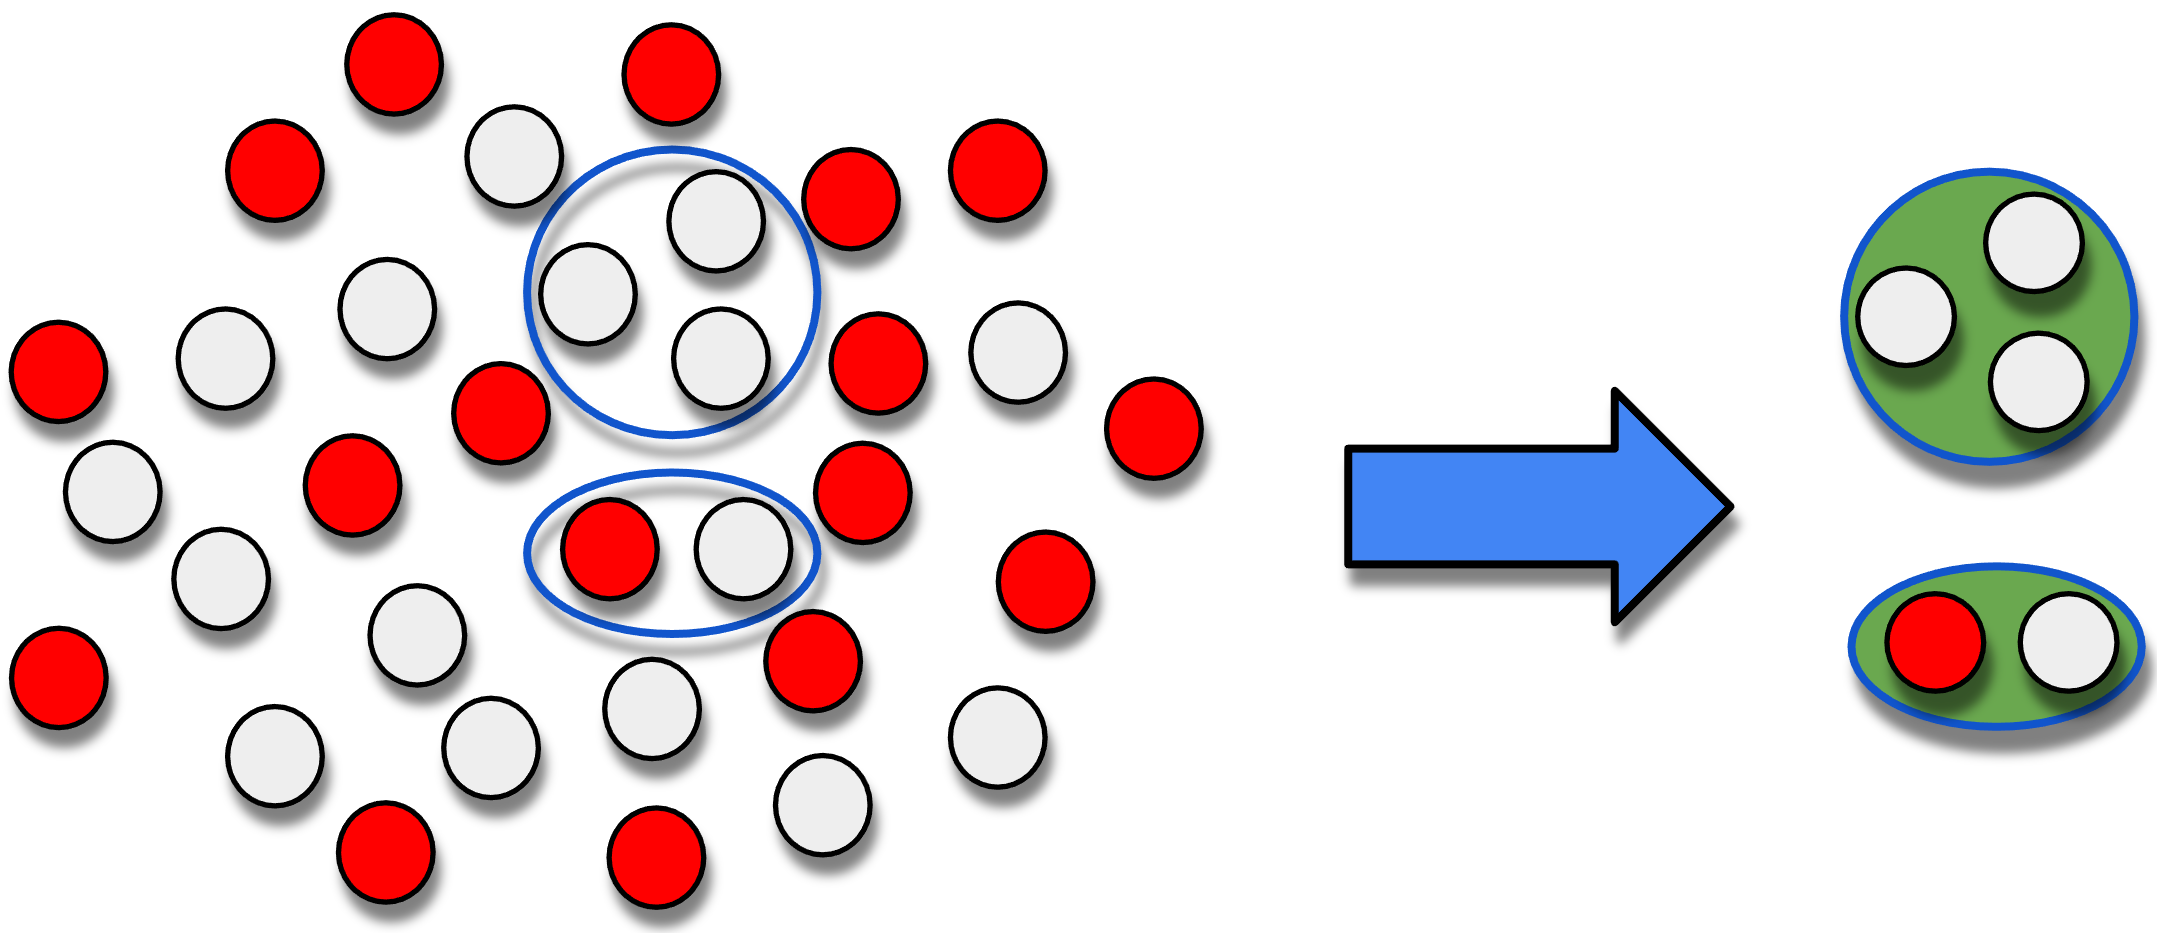
\includegraphics[width=0.7\linewidth]{Figures/Chapter 2/Coalescence.png}
    \caption{Representation of hadron production via recombination.}
\end{figure}

As outlined in Sec.~\ref{sec:high_pt}, the hadronisation process can be modified in the presence of a strongly-interacting deconfined medium. A novel mechanism for the production of hadrons, the recombination (also called coalescence), can take place in a thermalised system such as the QGP. When recombination occurs, two or three quarks close in the space-velocity phase space can bind together to form a hadron, which will have a higher (transverse-) momentum than the quarks that combined to form the hadron. This is different from the case of fragmentation, in which an energetic parton produces hadrons with lower momentum than the parent quark. As a consequence, the \pt distribution of hadrons formed by coalescence differs from the one expected from fragmentation. In particular, the hadron \pt is shifted to larger values as compared to fragmentation. Due to the steeply-falling quark \pt spectrum, this leads to a depletion of the low-\pt hadron yield, and an enhancement of the intermediate-\pt hadron yield. In addition, due to the relatively high abundance of low-\pt quarks and the sparsity of high-\pt partons, an enhancement of baryon-to-meson production-yield ratios at intermediate \pt is expected in proton-proton collisions when compared to \ee collisions as a natural consequence of the recombination mechanism. 

Models implementing the coalescence mechanism can effectively describe the production of hadrons in heavy-ion collisions. Intriguingly, models implementing recombination that successfully describe the production and azimuthal anisotropy of charm hadrons in these collisions, fail in doing so when this process is de-activated, as shown in Fig.~\ref{fig:D_recombination} for the case of prompt D mesons in the heavy-flavour sector. The D-meson \raa measured in the 0--10\% centrality interval and the second coefficient $v_2$ of the Fourier transform of the azimuthal distribution of D mesons in the 30--50\% centrality range measured by the ALICE Collaboration at midrapidity ($\lvert y\lvert<0.5$ for the \raa measurement and $\lvert y\lvert<0.8$ for that of the $v_2$ coefficients) at $\snn=5.02$~\tev~\cite{ALICE:2021rxa} are illustrated in the left and right panels, respectively. The measurements are compared to the Parton-Hadron-String Dynamics~\cite{Cassing:2008sv} (PHSD), POWLANG~\cite{Beraudo:2014boa}, and DAB-MOD~\cite{Katz:2019fkc} predictions, which are provided with (solid line) and without (dashed line) the implementation of the recombination process in the hadronisation mechanism. The calculations performed including the recombination of charm quarks with light quarks provide a good description of the experimental results, while they fail to reproduce the data when recombination is turned off. This suggests that the recombination mechanism plays a relevant role in the description of heavy-flavour hadron production in heavy-ion collisions.
\begin{figure}[htb]
  \centering
  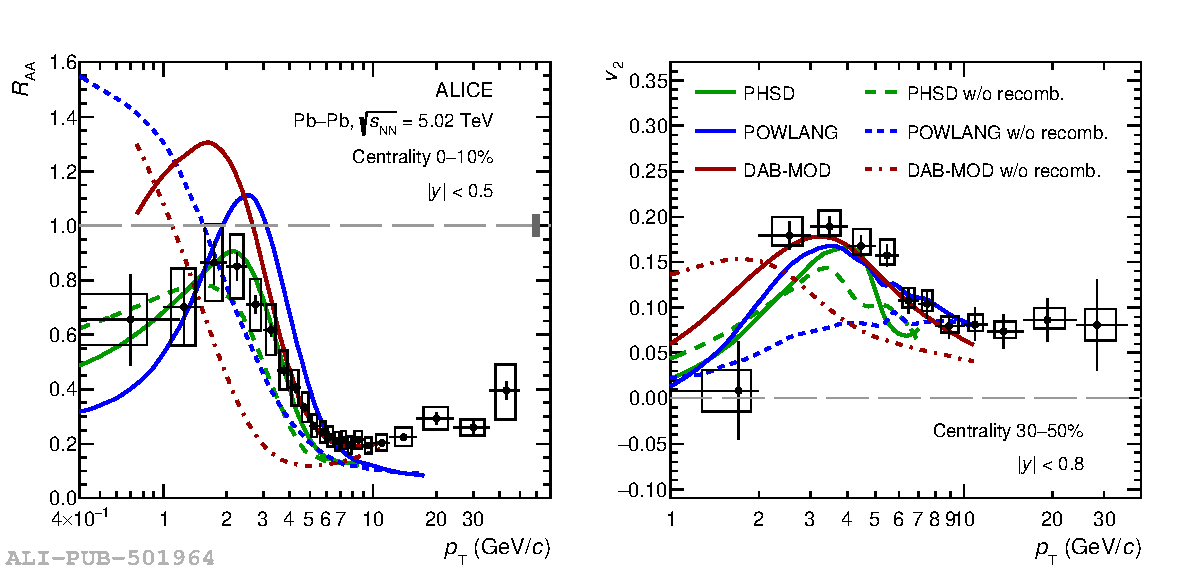
\includegraphics[width=\linewidth]{Figures/Chapter 2/D_Raa010_V23050_FragCoal_3models_1.pdf}
  \caption{Prompt D-meson $R_\mathrm{AA}$ in the 0--10\% centrality class (left panel) and $v_2$ in the 30--50\% centrality class (right panel) compared with predictions obtained with and without including hadronisation via recombination. Figure taken from Ref.~\cite{ALICE:2021rxa}.}
  \label{fig:D_recombination}
\end{figure}

New experimental measurements in pp and p--Pb collisions at the LHC~\cite{ALICE:2024ozd,ALICE:2016fzo,ALICE:2020wla,ALICE:2020wfu,ALICE:2021bli,CMS:2015fgy} provided a wealth of results suggesting that certain phenomena that are observed in nuclear collisions, such as strangeness enhancement and flow, may also occur in smaller collision systems. These effects are typically related to the presence of an expanding medium, thus raising the question of whether the coalescence hadronisation mechanism could also play a role in small collision systems. A hint that this could be the case comes from the observation that the production of charm baryons in pp and p--Pb collisions~\cite{ALICE:2022exq,ALICE:2024ozd} is significantly larger than expected from models based on a fragmentation tuned on \ee collisions. 

Various models have been developed in order to describe the observed charm-baryon enhancement in proton-proton and proton-lead collisions with the assumption of a recombination mechanism. These include the Quark (re-)Combination Mechanism~\cite{Song:2018tpv} (QCM) model, where coalescence between a charm quark and equal-velocity light quarks takes place at all momenta, and thermal weights are applied to account for relative production of scalar and vector mesons. In this model, the quark spectra are parametrised based on measurements of light-flavour hadrons and D-mesons. Other models adopt a description of the expanding system using a hydrodynamic approach and implementing hadronisation of the medium via a combination of coalescence and independent fragmentation. The Catania coalescence model~\cite{Minissale:2020bif} describes a thermalised system of u, d, s quarks, and gluons, where the charm quark can hadronise via either fragmentation or coalescence with light quarks from the bulk. The POWLANG model~\cite{Beraudo:2023nlq} predicts the formation of a small, deconfined, and expanding fireball in proton-proton collisions, where charm quarks are subject to rescattering and hadronisation, and can recombine with light quarks as in heavy-ion collisions. 

Each of these models provides a different hadronisation mechanism in proton-proton collisions compared to \ee ones, and independent hadronisation is no longer assumed. They improve the description of the data, achieving a better agreement with experimental results such as the \pt dependence of $\Lambda_\mathrm{c}^+/\mathrm{D}^0$ and $\Xi_\mathrm{c}^0/\mathrm{D}^0$ baryon-to-meson production-yield ratios.

\subsection{Core-corona model}
Core-corona models~\cite{Werner:2007bf} offer an intermediate approach between the two presented above. In these models, the fireball is divided into a high-density core part, treated with hydrodynamics and thermal modelling of particle production, similarly to that implemented in the SHM introduced in Sec.~\ref{subsec:SHM}, and a corona part, described using the Lund string model. This framework is based on the assumption that small QGP droplets may only be produced once the density is high enough. The EPOS Monte Carlo event generator~\cite{Porteboeuf:2008fgf} implements such a picture, and provides a very competitive description of data.

\subsection{Statistical hadronisation model}
The last model presented in this section exploits the idea of a thermalised system, which is by definition in thermal equilibrium. A macroscopic approach to hadronisation, based on a statistical model, can be used to describe the charm-hadron production in hadronic collisions. The principles of thermodynamics can be applied to the hadronisation process, where the hadron yields are determined by the hadron's mass and the temperature and baryon chemical potential of the system. As described in Sec.~\ref{subsec:SHM}, this approach has been successfully adopted to describe the light and strange hadron production in heavy-ion collisions and smaller systems. 

Different approaches are used to predict the production of light- and heavy-flavour hadrons with the SHM. Due to the large masses of charm and beauty quarks, which are significantly larger than the temperature of the QGP, their thermal production in the medium is strongly suppressed. Therefore, the production of charm and beauty quarks is determined by their initial production in the hard-scattering processes. Their distribution into hadrons is then predicted with thermal weights. A charm balance equation is used to ensure the conservation of the initially produced charm quarks into the final-state hadrons via a fugacity factor $g_\mathrm{c}$, which accounts for the absence of chemical equilibrium for heavy quarks. In addition, the description of heavy-flavour hadron production and the baryon enhancement in this framework requires the inclusion of a strong feed-down from an augmented set of excited charm- or beauty-baryon states, not included in the PDG~\cite{pdg}. Recent model developments~\cite{He:2019tik,He:2022tod} have extended the Statistical Hadronisation Model (SHM) to include a set of 18 $\mathrm{\Lambda_c}$'s, 42 $\mathrm{\Sigma_c}$'s, 62 $\mathrm{\Xi_c}$'s, and 34 $\mathrm{\Omega_c}$'s excited states up to a mass of 3.5~\gev, predicted by the Relativistic Quark Model~\cite{Ebert:2011kk}. Such models provide a good description of the measured $\mathrm{\lc/D^0}$ production yield ratio and the \pt spectra of D mesons and \lc at midrapidity.

\subsection{Baryon enhancement: \texorpdfstring{$\mathrm{\lc/D^0}$}{Lc/D0} ratio}
\begin{figure}[htb]
    \centering
    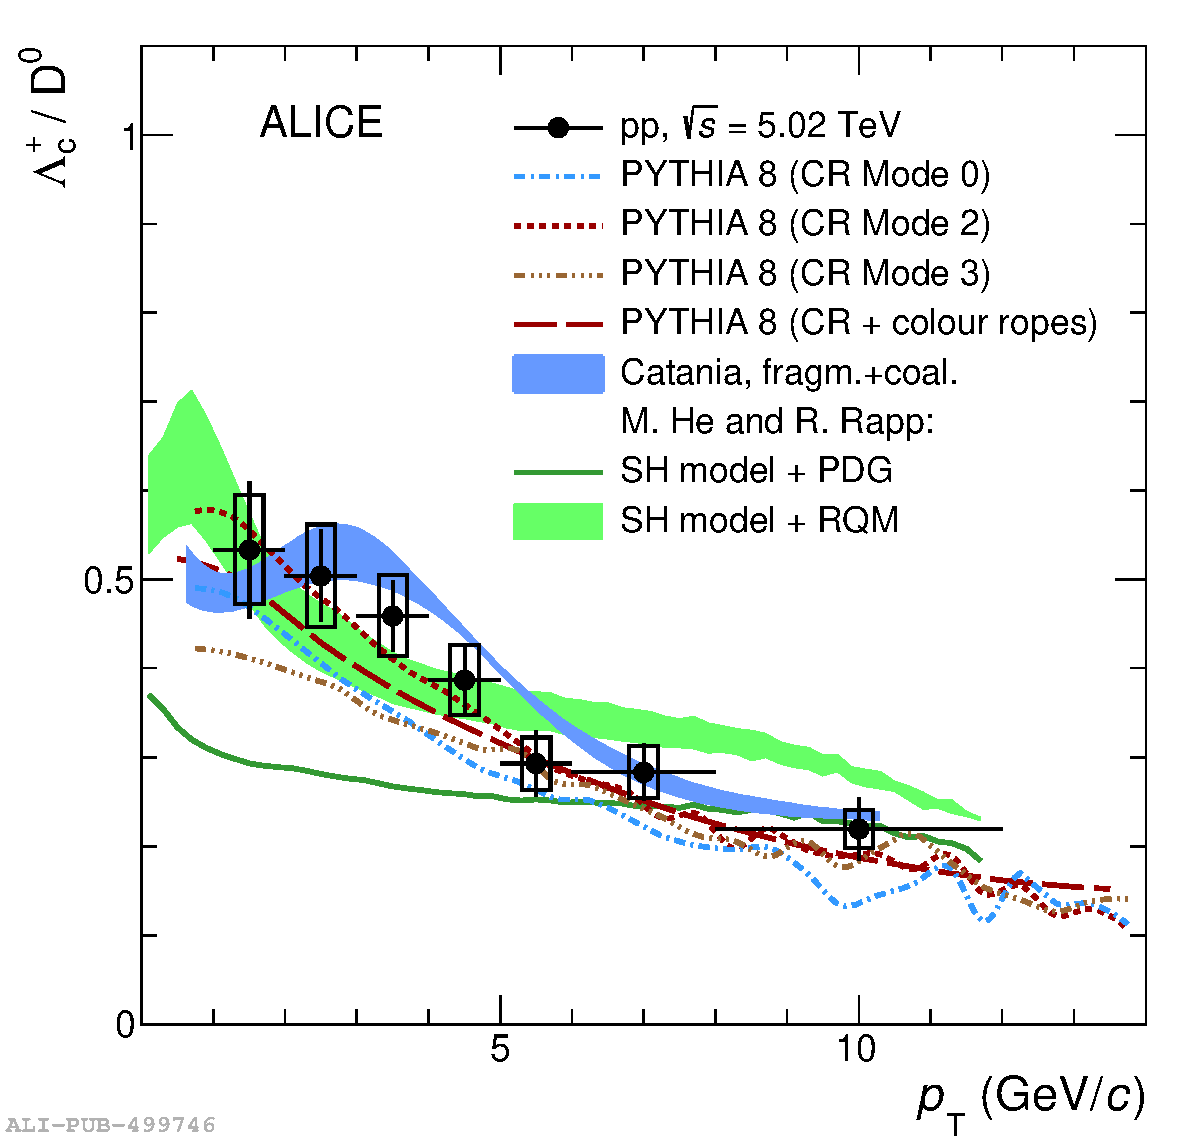
\includegraphics[width=0.48\linewidth]{Figures/Chapter 2/LcD_models_withModifiedModels_ropes_coal_2.pdf}
    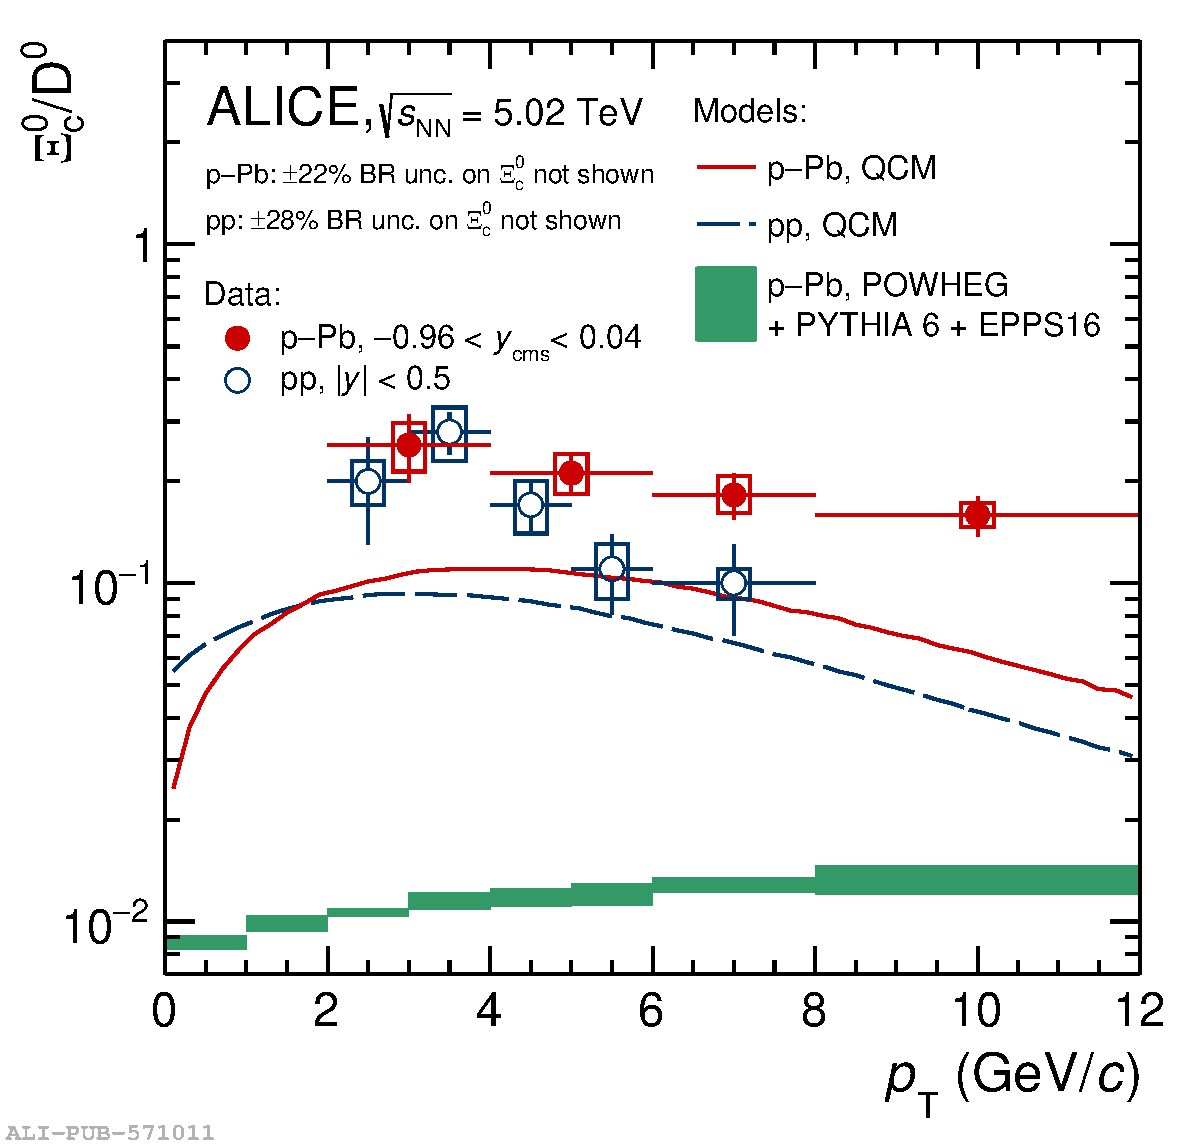
\includegraphics[width=0.48\linewidth]{Figures/Chapter 2/Xic0_D0_Ratio.pdf}
    \caption{Left panel: $\mathrm{\lc/D^0}$ production-yield ratio measured at midrapidity ($\lvert y\rvert < 0.5$) in pp collisions at $\sqrt{s} = 5.02$~\tev by the ALICE Collaboration~\cite{ALICE:2020wla} as a function of \pt, compared to theoretical predictions. Right panel: $\mathrm{\Xi_c^0/D^0}$ production-yield ratio measured at midrapidity ($-0.96 < y < 0.05$) in p--Pb collisions at $\snn = 5.02$~\tev by the ALICE Collaboration~\cite{ALICE:2020wla} as a function of \pt, compared to theoretical predictions. Figures taken from Refs.~\cite{ALICE:2020wla} and~\cite{ALICE:2024ozd}.}
    \label{fig:Lambda_c_D0}
\end{figure}
The hadronisation process can be experimentally studied through the measurement of production-yield ratios of hadrons. Since the initial state of the collision and the charm production cross-section is the same for all charm hadrons, the measurement of the production-yield ratio of different charm hadrons can be expressed, using the factorisation theorem, as the ratio of the fragmentation functions of the hadrons, which describe the hadronisation process. 

The left panel of Fig.~\ref{fig:Lambda_c_D0} shows the $\mathrm{\lc/D^0}$ baryon-to-meson production-yield ratio measured at midrapidity ($\lvert y\rvert < 0.5$) in pp collisions at $\sqs = 5.02$~\tev by the ALICE Collaboration as a function of \pt, compared to models that include mechanisms to enhance baryon production compared to those in which the hadronisation is implemented through independent fragmentation and parametrised on results from \ee collisions, already presented in Fig.~\ref{fig:Lambda_c_D0_ee}. They include i) \textsc{Pythia}~8 simulations with colour-reconnection beyond the leading-colour approximation~\cite{Christiansen:2015yqa} (three colour reconnection modes (0,2,3), which apply different constraints on the allowed reconnection are considered); ii) \textsc{Pythia}~8 with colour-reconnection plus rope hadronisation~\cite{Bierlich:2014xba} where colour charges can act coherently to form a rope, increasing the effective string tension; iii) Catania coalescence model~\cite{Minissale:2020bif}, where a QGP is formed in pp collisions and hadronisation occurs through both recombination and fragmentation; iv) SHM~\cite{Braun-Munzinger:2003pwq} where the underlying charm baryon spectrum is either taken from the PDG~\cite{pdg}, or augmented to include additional excited baryon states, which have not yet been observed but are predicted by the RQM~\cite{Ebert:2011kk}. These models are capable of describing both the magnitude and the \pt dependence of the $\mathrm{\lc/D^0}$ ratio, suggesting that the hadronisation process in proton-proton collisions might differ from that in \ee collisions. This conclusion is also confirmed by the measurement of the $\mathrm{\Xi_c^0/D^0}$ baryon-to-meson production-yield ratio at midrapidity ($-0.96<y<0.04$) in p--Pb collisions at $\snn = 5.02$~\tev performed by the ALICE Collaboration~\cite{ALICE:2024ozd}, shown in the right panel of Fig.~\ref{fig:Lambda_c_D0}. The measured ratio is compared to POWHEG~\cite{Frixione:2007nw} NLO pQCD calculations, matched with \textsc{Pythia}~6~\cite{Sjostrand:2006za} to generate the parton shower and fragmentation, which is tuned on \ee collisions, and to the EPPS16  parametrisation of the modification of the PDFs in the nuclear environment of the lead ion~\cite{Eskola:2016oht}. It predicts a slightly increasing trend with \pt, and undershoots the measured $\mathrm{\Xi_c^0/D^0}$ by a large factor of around 20. Predictions from the QCM model~\cite{Song:2018tpv} implementing a coalescence hadronisation mechanism provide a better description of both the \pt dependence and the magnitude of the data. 

The influence of the surrounding environment in the hadronisation of the charm quark could also potentially affect the relative abundances of strange and non-strange charm hadrons with increasing multiplicity from  \ee collisions to high multiplicity proton-proton and proton-nucleus collisions. Enhanced production of charm-strange hadrons may result from the coexistence of numerous strange quarks (which could be thermally produced in an environment with $T \gg m_\mathrm{s}$, as explained in Sec.~\ref{subsec:StrangenessEnhancement}) within the same region as the charm quark, thereby increasing the probability of recombination between them. This phenomenon can be studied through the measurement of the production-yield ratio of charm-strange hadrons to non-strange charm hadrons, such as the $\mathrm{D_s^+}$-meson to $\mathrm{D^+}$-meson ratio, which constitutes the primary focus of this Thesis.